\chapter{Results}
\section*{Motion Estimation}
\begin{figure}
    \centering
    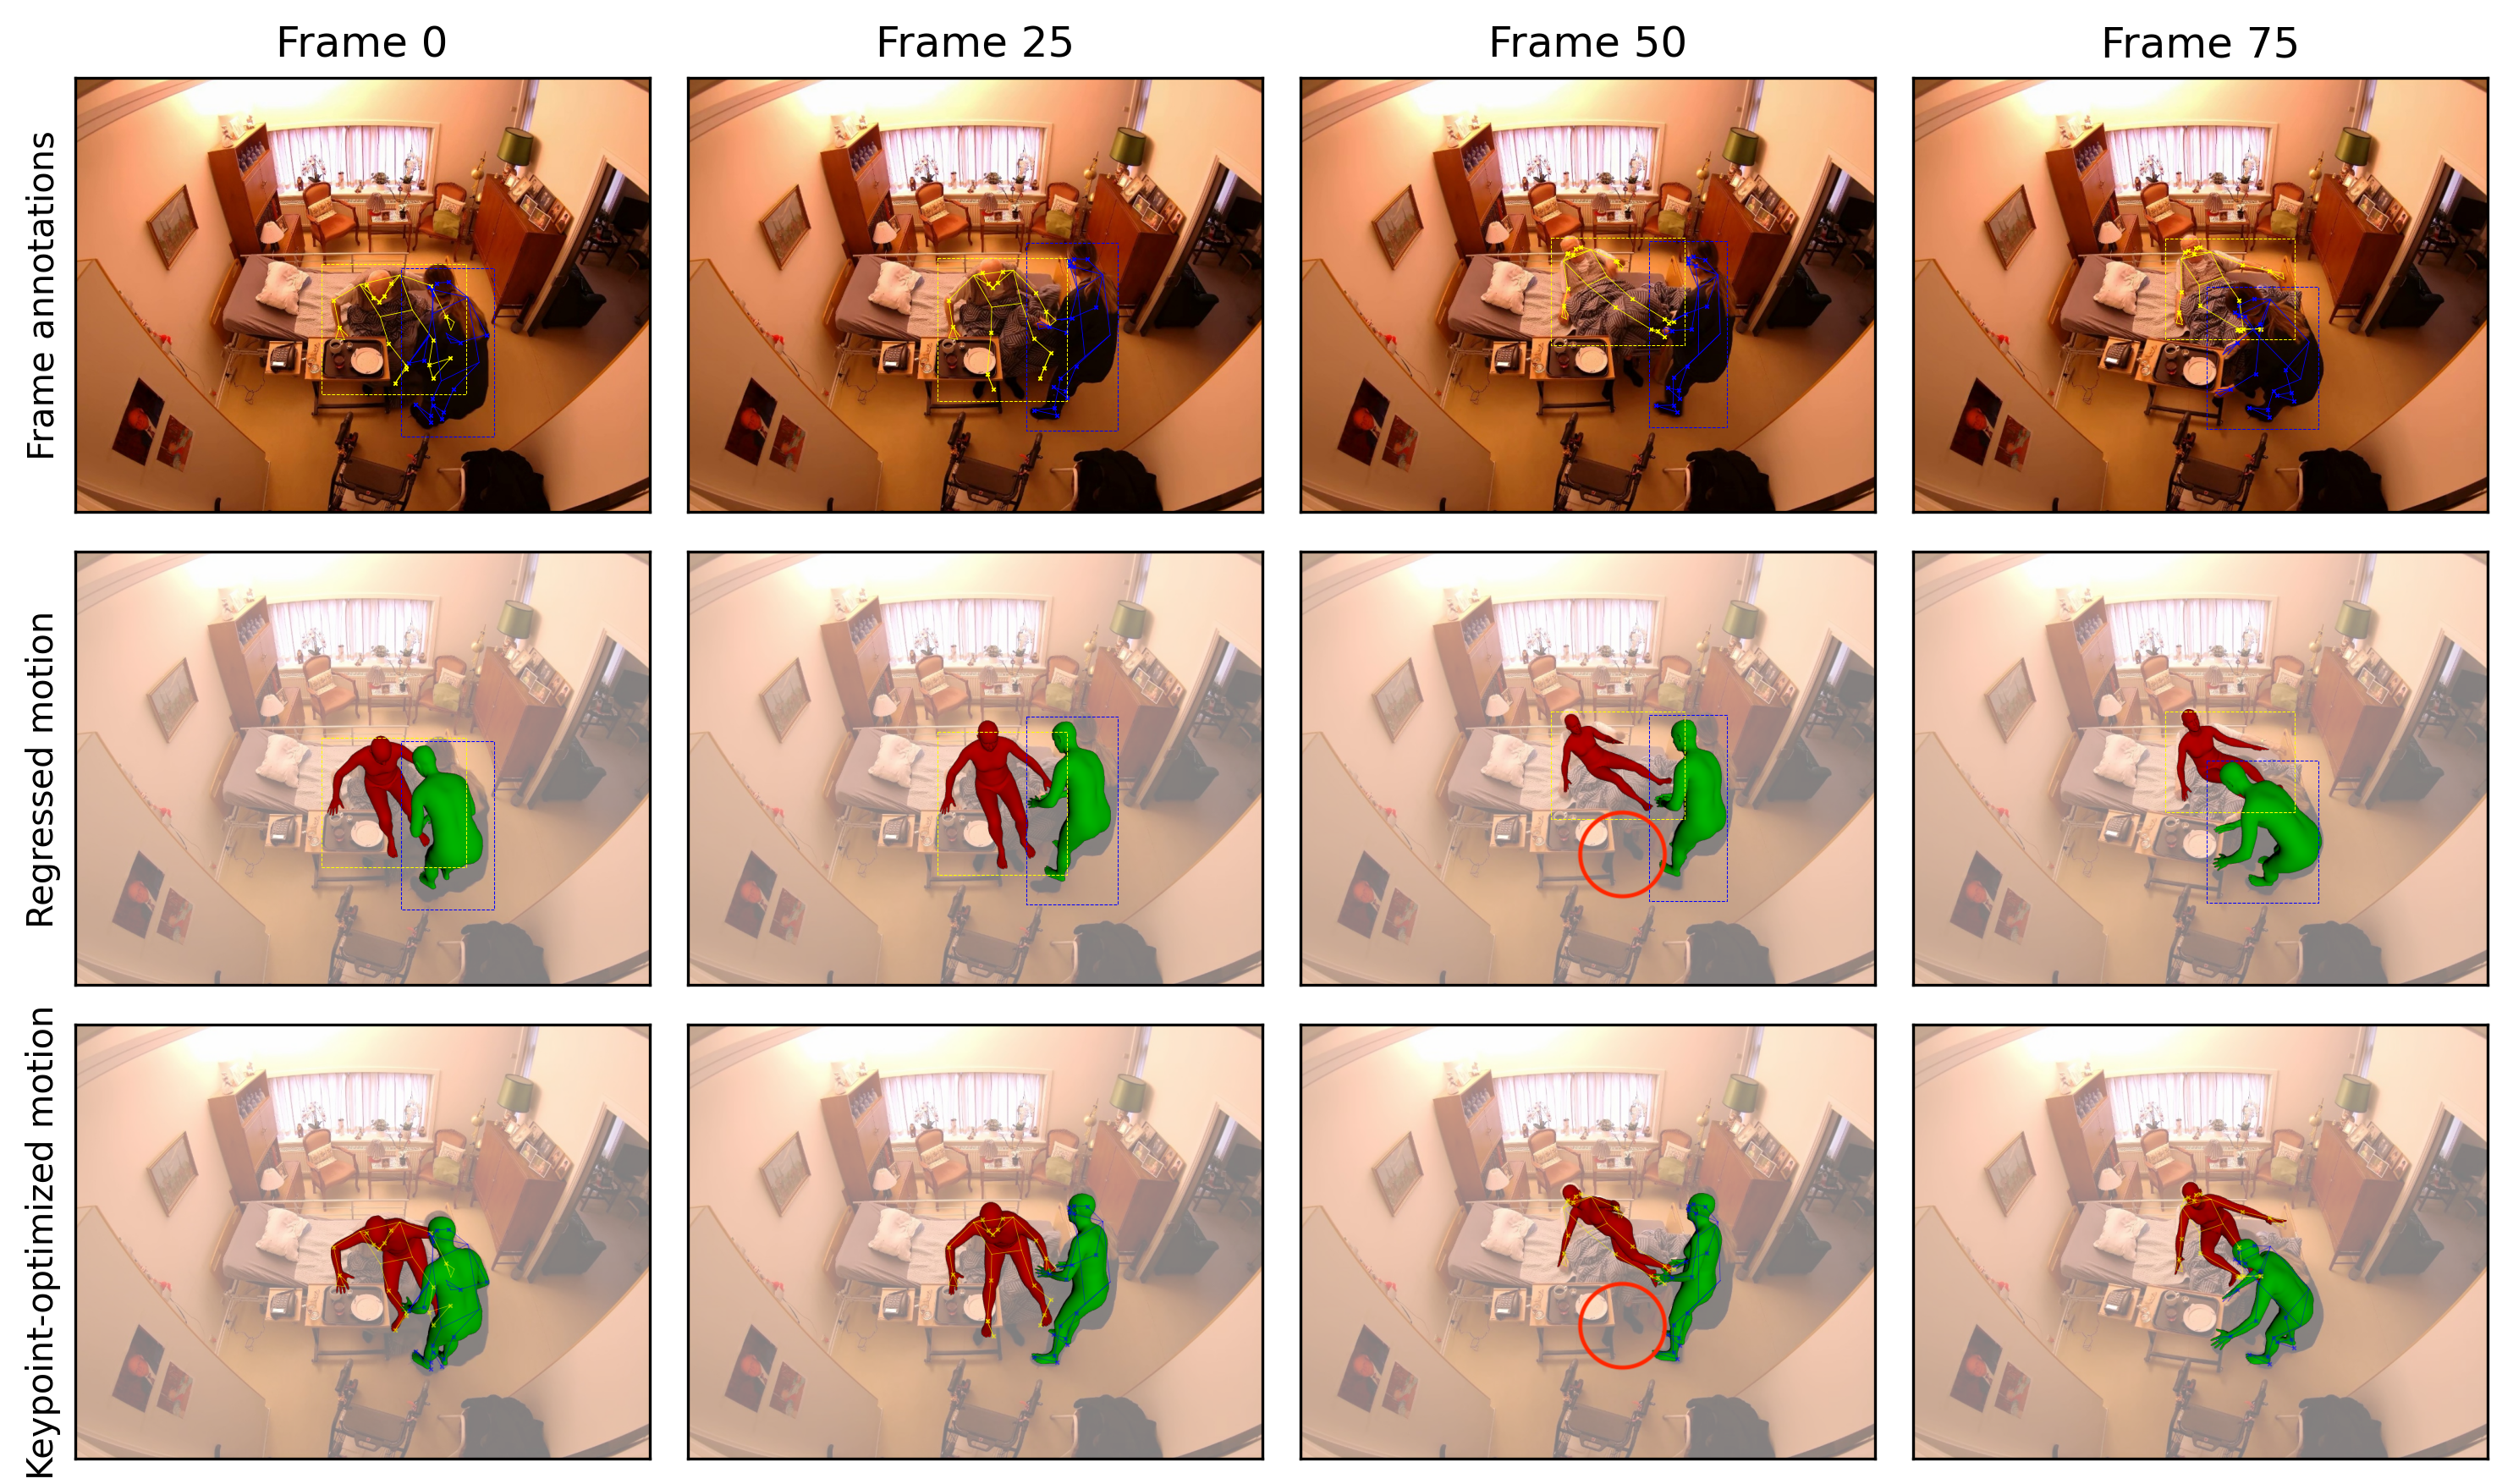
\includegraphics[width=\linewidth]{figures/results/motion1.png}
    \caption{Example of bad annotations effect on estimated motion.}
    \label{fig:motion1}
\end{figure}

\begin{figure}
    \centering
    \includegraphics[width=\linewidth]{figures/results/motion2.png}
    \caption{Local optimum of optimization-based method and hybrid method.}
    \label{fig:motion2}
\end{figure}

\begin{figure}
    \centering
    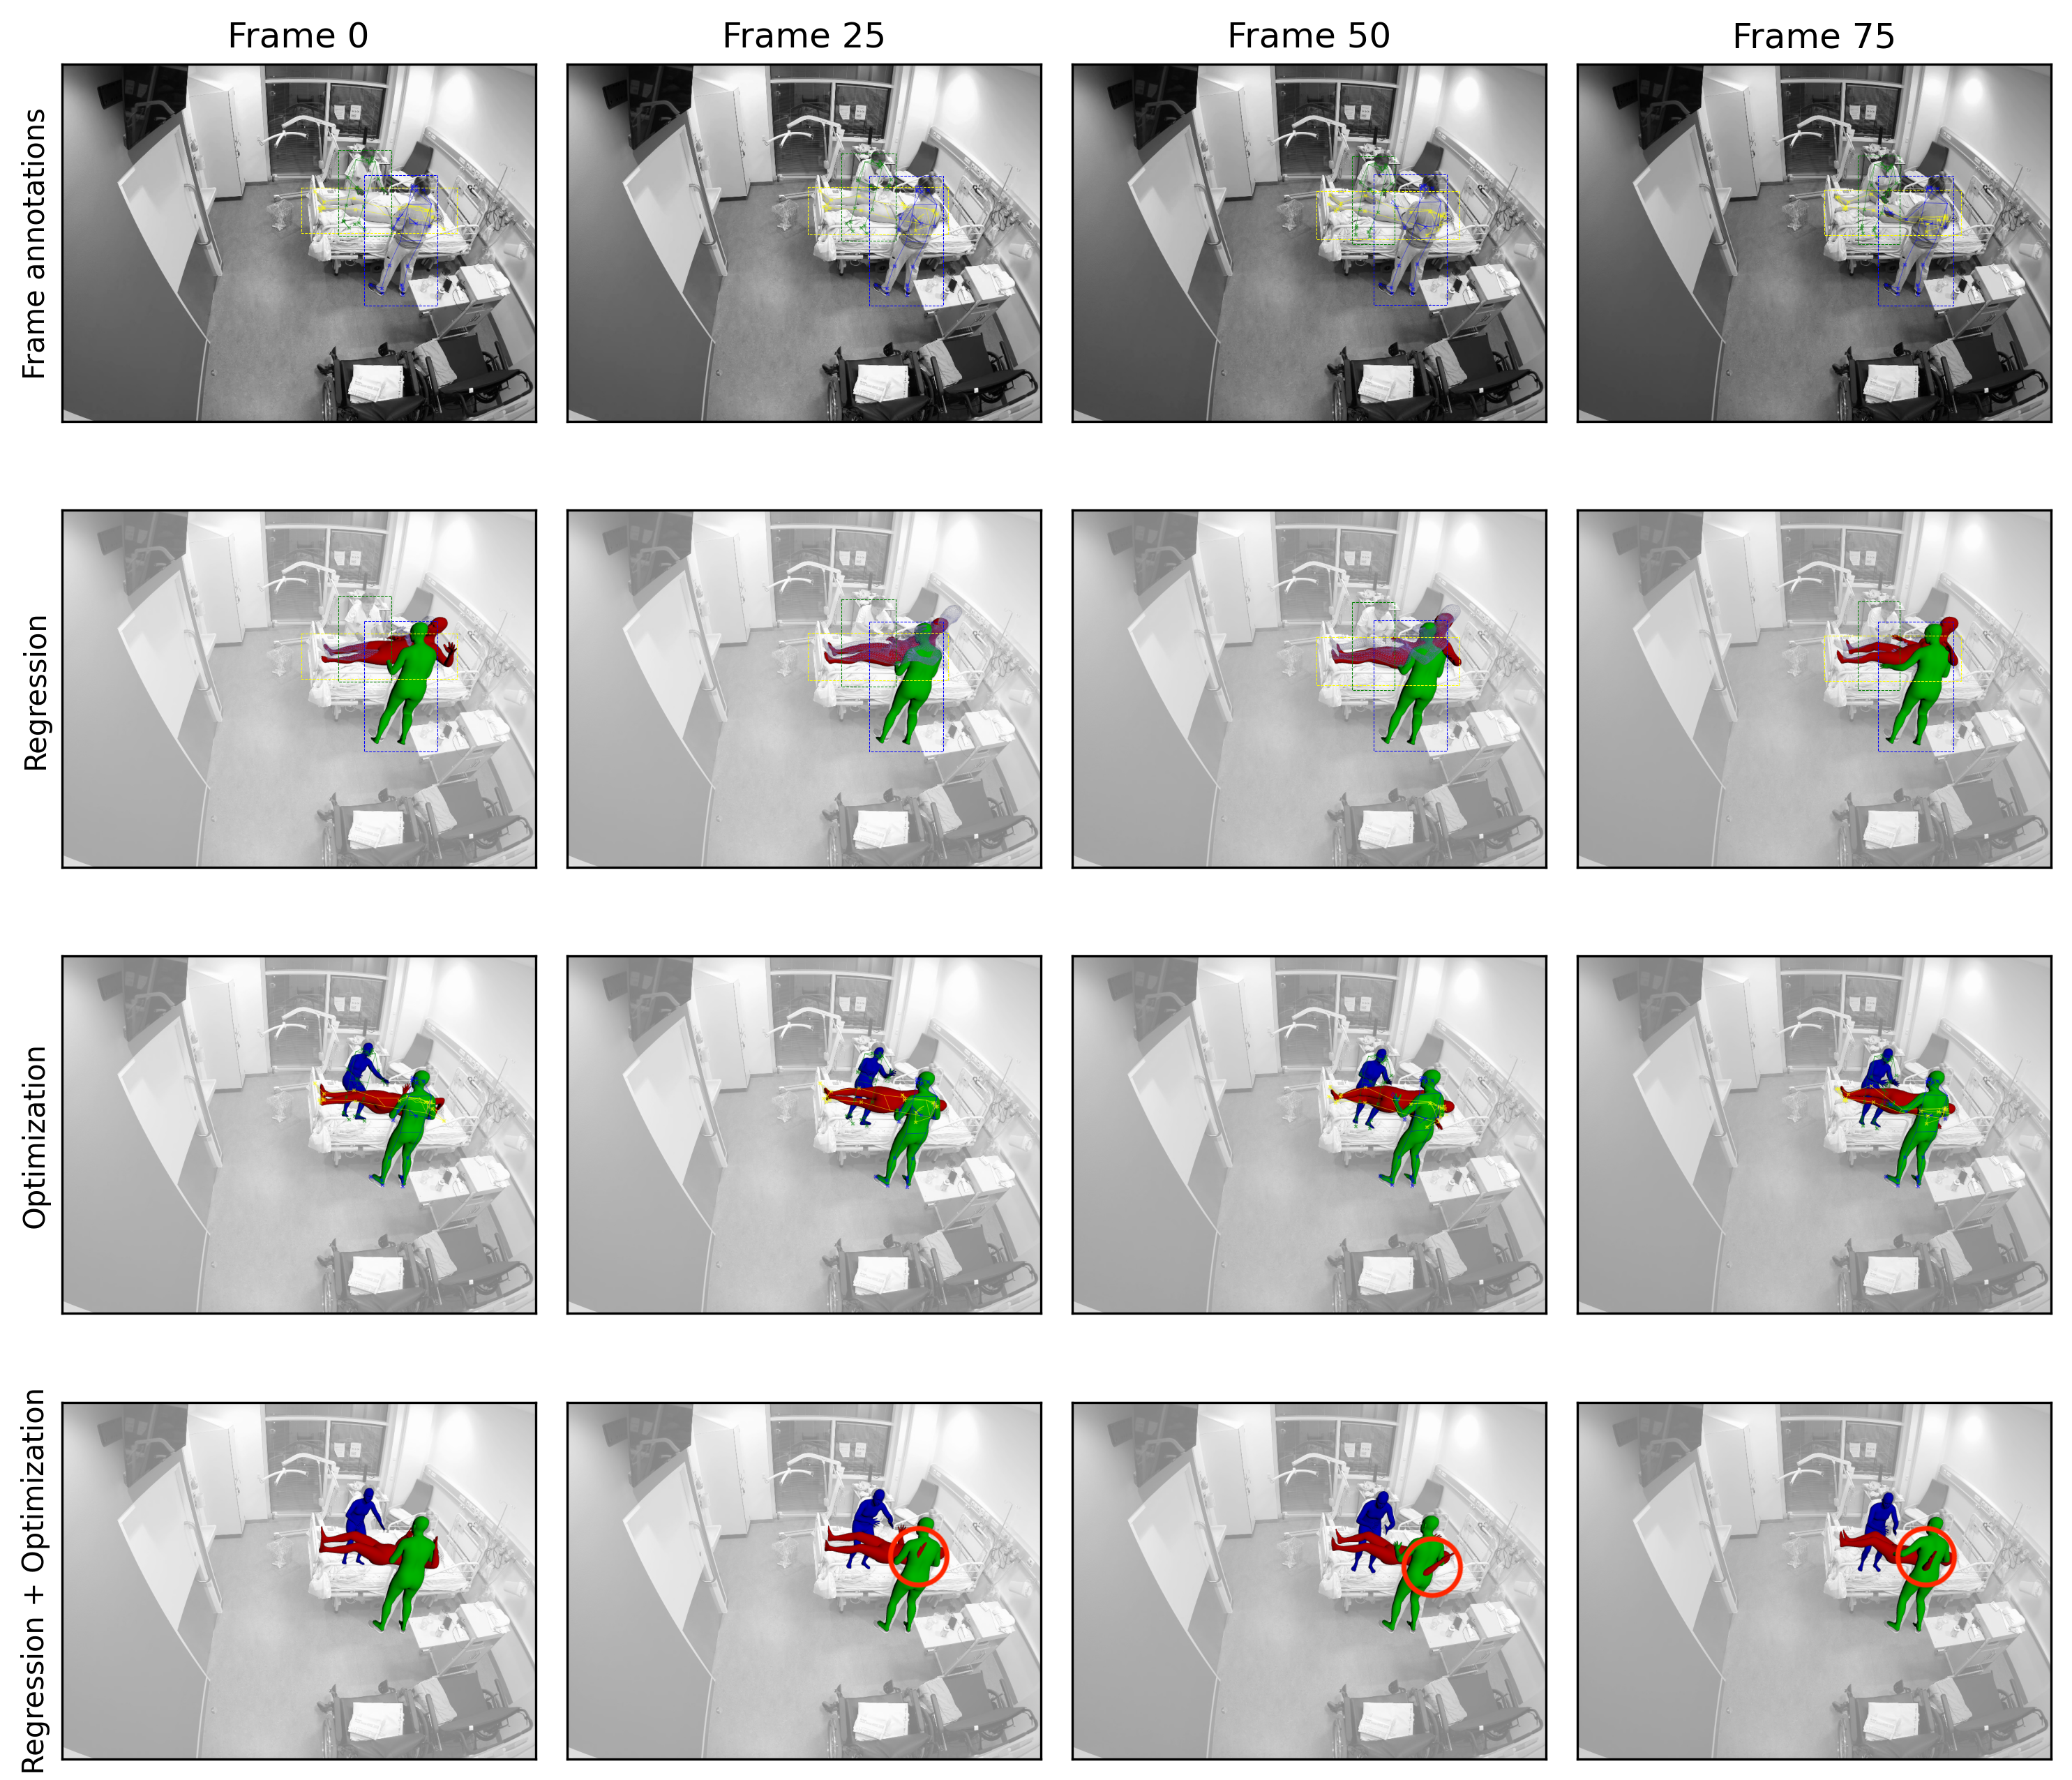
\includegraphics[width=\linewidth]{figures/results/motion3.png}
    \caption{Interpenetration between different people.}
    \label{fig:motion3}
\end{figure}

In the example shown in \cref{fig:motion1}, we notice that the keypoints do not correspond to the actual joints of the person. Specifically, the leg keypoints appear to be incorrectly marked as if the legs were covered by a blanket, despite being visible in the image, as indicated by the red ring. This might be an error in the keypoint annotations, either due to the autolabelling step in the pipeline failing to correctly detect the keypoints or a lack of human attention. As a result, the optimized pose (red) diverges from the actual pose of the person, while the green person's pose looks consistent with the person in the frame. Interestingly, the regressed pose also estimates the legs as being covered by the blanket, although it predicts the pose directly from the image. This again seems to be a result of a bad bounding box segmentation, not including the legs.

A common encountered problem with the optimization-based method is seen in \cref{fig:motion2}, where the optimized pose appears to be stuck in a local optimum during the optimization phase. In contrast, the regression-based method seems to correctly predict the pose but either overestimates the size of the person or places the person too close to the camera. Inspecting the outline of the person in the first frame indicates that the regression-based method might be sensitive to clothing or body shape. Initializing the pose from the regression estimates and then optimizing against the keypoints seems to give the best pose fit. 

As each pose is optimized in isolation, artifacts such as interpenetration might occur, as observed in the last row of \cref{fig:motion3}, after optimizing the initial regression-based estimate to align with the keypoints. Furthermore, the regression-based method fails to detect the occluded nurse behind the bed, as indicated by the semi-transparent mesh, indicating that the pose was removed due to closer matching the keypoints of the laying patient (see \cref{section:regression-pose-estimation}).

% \begin{figure}[H]
%     \centering
%     \includegraphics[width=\linewidth]{figures/results/motion4.png}
%     \caption{Example of bad ground truth kpts.}
% \end{figure}

% \begin{figure}[H]
%     \centering
%     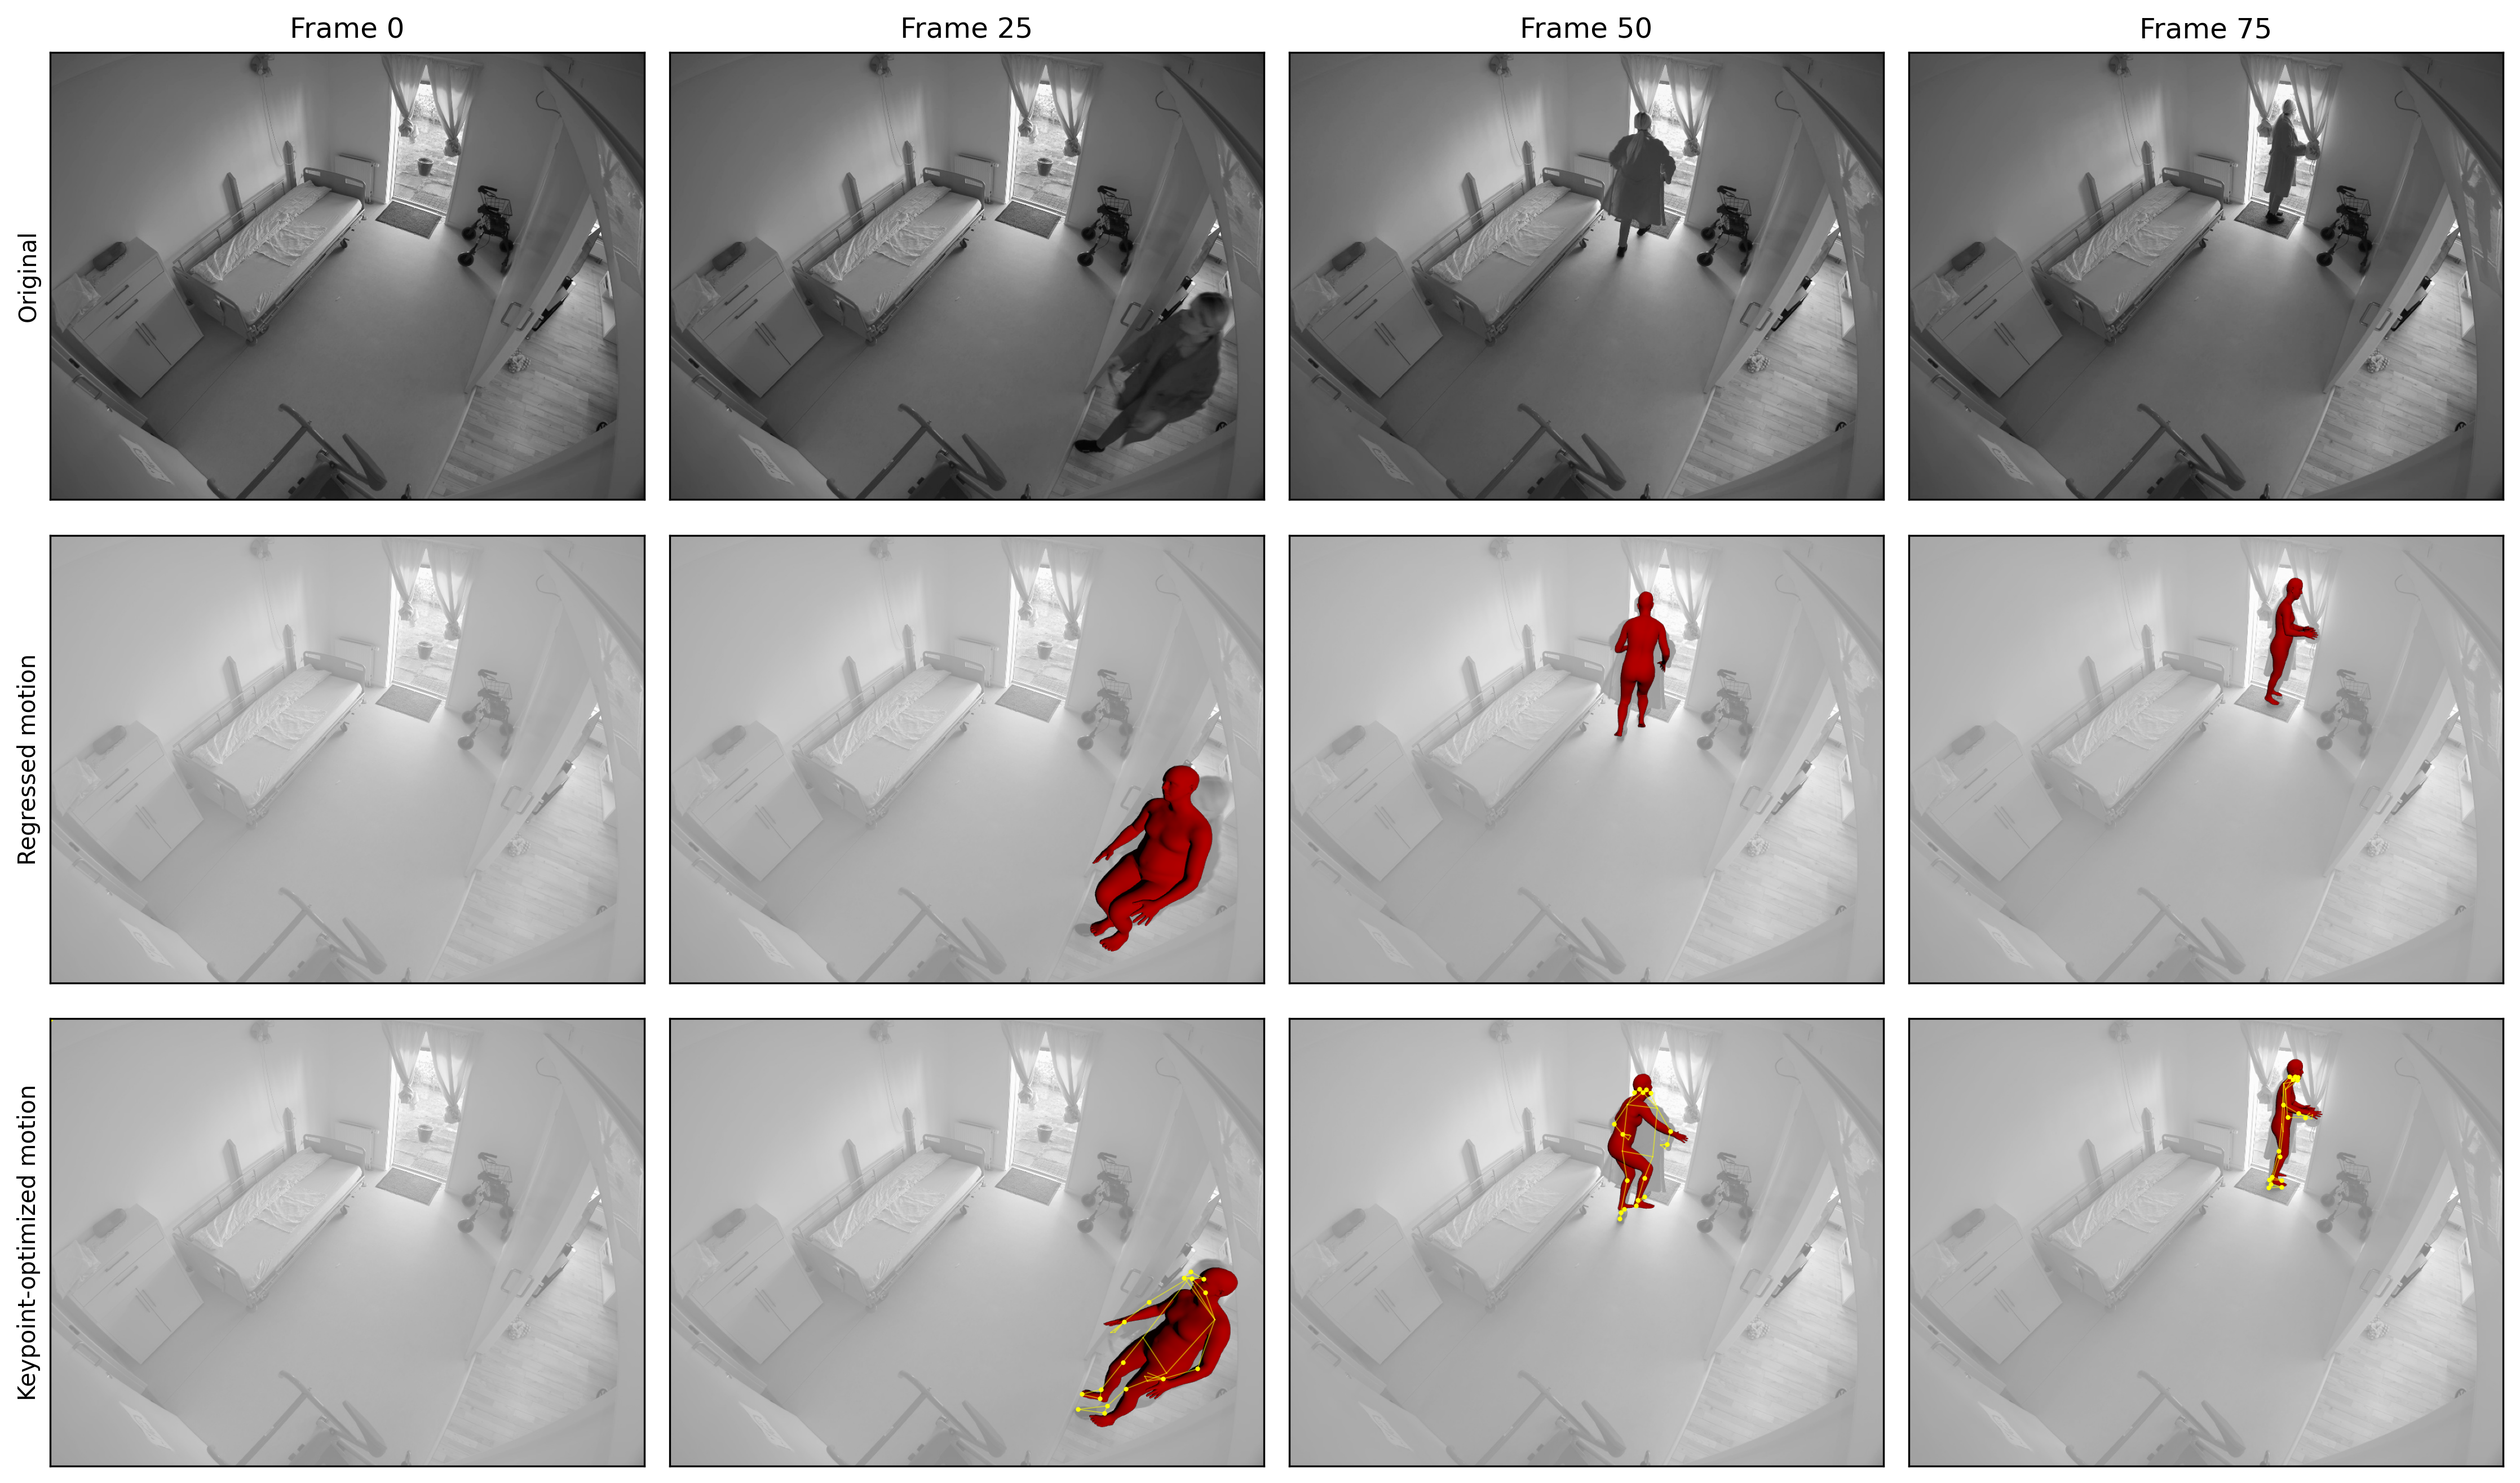
\includegraphics[width=\linewidth]{figures/results/motion5.png}
%     \caption{Example of bad ground truth kpts.}
% \end{figure}

\section*{Single-Human Motion Generation}

\begin{figure}
    \centering
    \begin{subfigure}{0.32\linewidth}
        \includegraphics[width=\linewidth]{figures/results/single-kick1.png}
    \end{subfigure}
    \hfill
    \begin{subfigure}{0.32\linewidth}
        \includegraphics[width=\linewidth]{figures/results/single-kick2.png}
    \end{subfigure}
    \hfill
    \begin{subfigure}{0.32\linewidth}
        \includegraphics[width=\linewidth]{figures/results/single-kick3.png}
    \end{subfigure}
    \caption{Three examples of single motion generation with prompt: \textit{"A person kicks with their left leg."}}
\end{figure}

\begin{figure}
    \centering
    \begin{subfigure}{0.32\linewidth}
        \includegraphics[width=\linewidth]{figures/results/single-runs1.png}
    \end{subfigure}
    \hfill
    \begin{subfigure}{0.32\linewidth}
        \includegraphics[width=\linewidth]{figures/results/single-runs2.png}
    \end{subfigure}
    \hfill
    \begin{subfigure}{0.32\linewidth}
        \includegraphics[width=\linewidth]{figures/results/single-runs3.png}
    \end{subfigure}
    \caption{Three randomly picked examples of generated motion with prompt: \textit{"A man runs to the right then runs to the left then back to the middle."}}
\end{figure}


\begin{figure}
    \centering
    \begin{subfigure}{0.32\linewidth}
        \includegraphics[width=\linewidth]{figures/results/single-falls1.png}
    \end{subfigure}
    \hfill
    \begin{subfigure}{0.32\linewidth}
        \includegraphics[width=\linewidth]{figures/results/single-falls2.png}
    \end{subfigure}
    \hfill
    \begin{subfigure}{0.32\linewidth}
        \includegraphics[width=\linewidth]{figures/results/single-falls3.png}
    \end{subfigure}
    \caption{Three randomly picked examples of generated motion with prompt: \textit{"A persons loses balance and falls to the ground."}}
\end{figure}

\section*{Multi-Human Motion Generation}

\begin{figure}
    \centering
    \includegraphics[width=\linewidth]{figures/results/multi-passion.png}
    \caption{Prompt: \textit{"With fiery passion two dancers entwine in Latin dance sublime."}}
\end{figure}


\begin{figure}
    \centering
    \includegraphics[width=\linewidth]{figures/results/multi-selfie1.png}
    \caption{Prompt: \textit{"With merry smiles the two snap their selfie."}}
\end{figure}


\begin{figure}
    \centering
    \includegraphics[width=\linewidth]{figures/results/multi-pick-up.png}
    \caption{Prompt: \textit{"Two people picking up something from the ground."}}
\end{figure}